\documentclass[12pt]{article}
\usepackage[utf8]{inputenc}
\usepackage{natbib}
\usepackage{graphicx}
\usepackage[portuguese]{babel}

\title{IF672 - Algoritmos e Estruturas de Dados}
\author{Pedro Augusto de Almada Lobo Fonseca}
\date{Dezembro 2021}

\begin{document}
\maketitle

\begin{figure}[h]
    \centering
    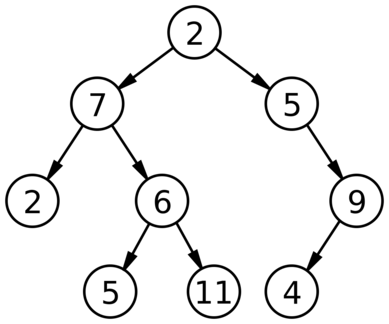
\includegraphics{images/binarytree.png}
    \caption{Árvore binária, um dos principais tipos de estrutura de dados.} \cite{binarytree}
    \label{fig:binarytree}
\end{figure}

\section{Introdução}
O objetivo desta disciplina é estudar estruturas de dados para que se possa aprender a escrever programas mais eficientes. A busca por tal eficiência, no entanto, não deve entrar em conflito com o design e a clareza do código \cite{CInWiki_algoritmos}. Um algoritmo nada mais é do que uma sequência finita de instruções executáveis, explícitas e não ambíguas que visam obter uma solução para um determinado tipo de problema \cite{algoritmo}. Por sua vez, uma estrutura de dados é uma coleção tanto de valores (e seus relacionamentos) quanto de operações (sobre os valores e estruturas decorrentes) \cite{estrutura_de_dados}. Na prática, estrutura de dados se refere à forma com a qual se organiza dados na memória de um computador. Ao final deste curso, o aluno terá desenvolvido não só um repertório básico de estruturas de dados e algoritmos, mas também a capacidade de analisar a eficiência de um algoritmo ou de uma estrutura de dados, tanto em termos de tempo quanto de memória.

\section{Relevância}
Por que os programas devem ser eficientes quando os novos computadores ficam mais rápidos a cada ano? A razão é que as ambições humanas crescem proporcionalmente às capacidades da tecnologia. Destarte, em vez de tornar as necessidades de eficiência obsoletas, o desenvolvimento do poder de computação e da capacidade de armazenamento tende a aumentar as apostas de eficiência à medida que são experimentadas tarefas mais complexas. Além disso, a maioria dos currículos de ciência da computação reconhece que as boas habilidades de programação começam com uma forte ênfase nos princípios fundamentais de engenharia de software. Assim, uma vez que um programador aprendeu os princípios de design e implementação de programas claros, o próximo passo é estudar os efeitos da organização de dados e algoritmos sobre a eficiência do programa.  \cite{CInWiki_algoritmos}

\section{Relação com outras disciplinas}
Por ser uma disciplina lecionada no 2º período \cite{CInWiki}, ela tem como único pré-requisito:
\begin{itemize}
    \item IF669 - Introdução à Programação
\end{itemize}
No entanto, ela é uma das cadeiras mais fundamentais do curso de ciência da computação e é pré-requisito das seguintes disciplinas obrigatórias:
\begin{itemize}
    \item IF682 - Engenharia de Software e Sistemas
    \item IF685 - Gerenciamento de Dados e Informação
    \item IF689 - Informática Teórica
    \item IF684 - Sistemas Inteligentes
\end{itemize}

\bibliographystyle{plain}
\bibliography{references}

\end{document}